\section{Anforderungen}

\subsection{Personas}
Unter der Definition von Personas\footcite{persona_definition} versteht man: 
\begin{displayquote}
Personas (lat. Maske) sind Nutzermodelle, die Personen einer Zielgruppe in ihren Merkmalen charakterisieren. Sie können z. B. einem Entwicklerteam aufgrund ihrer umfangreichen Beschreibung helfen, sich in die Lage der potenziellen Nutzer zu versetzen und diese Perspektive während des gesamten Designprozesses leicht zu vertreten. Sie werden mit einem Namen, einem Gesicht, einer Funktion, einem Werdegang und einem Privatleben versehen. Personas verfügen über Ziele und Verhaltensweisen, haben Vorlieben und Erwartungen.
\end{displayquote}

Diese Personas wurden erstellt, um ein klareres Bild vermitteln zu können, welche Funktionalitäten durch den Aufgaben-Coach ermöglicht werden und wie diese Anwendung eingesetzt werden könnte.

\subsubsection{Persona 1}
\subsubsection*{Persönliches Profil}
Abirsana ist Lehrerin an der Schule Gossau und unterrichtet die Fächer Mathematik, Deutsch und Englisch.

\subsubsection*{Situation}
Um den Unterricht interessanter zu gestalten, greift Abirsana oft auf digitale Medien, wie zum Beispiel YouTube Videos, zurück. Oftmals ist jedoch das Material nicht genau auf den Schulstoff angepasst oder die Qualität lässt zu wünschen übrig. Zudem braucht sie sehr lange, um passende Videos zu finden.

\subsubsection*{Szenario}
Im Rahmen des Unterrichts soll es Abirsana möglich sein, die Aufgaben-Coach Webanwendung zu verwenden. Sie soll in der Lage sein, einzelne Fächer und Theorieinhalte ihrer Klasse zur Verfügung zu stellen. Zudem kann sie eigene Übungen erfassen, welche die Schüler auch gleich über die Webanwendung lösen. Sind die Aufgaben abgegeben, kann sie die einzelnen Aufgaben anschauen und bewerten. Falls ihr auffällt, dass ein gewisser Schüler oder die ganze Klasse etwas nicht versteht, kann sie so direkt die Wissenslücke schliessen.

\subsubsection{Persona 2}
\subsubsection*{Persönliches Profil}
Salina ist Schülerin an einer Schule. Seit längerer Zeit hat sie jedoch Mühe mit dem Schulstoff und ihre Noten sind auch nicht mehr so gut.

\subsubsection*{Situation}
Salina versteht oft nichts, wenn ihr Lehrer ihr etwas erklärt. Zu Hause verbringt sie dann viel Zeit im Internet, um einzelne Themen zu lernen. Sie hat aber weder die Zeit noch die Lust dazu, zu Hause nochmals die gesamte Theorie anschauen zu müssen und nach guten Videos zu suchen.

\subsubsection*{Szenario}
Nach kurzer Zeit hat Salina die Lehrer an ihrer Schule dazu überredet, die Aufgaben-Coach Plattform einzusetzen. Somit ist Salina freier im Lernen. In der Schule kann sie sich selbstständig ein Thema beibringen. Falls sie dennoch etwas nicht versteht, kann sie direkt auf eine Lehrperson zugehen, welche ihr dann das Kapitel vielleicht noch etwas genauer erklärt. \\
Zudem wird sie nicht von anderen Schülern aufgehalten, weil diese länger brauchen, um ein Thema zu lernen. Zu Hause verbringt sie auch nicht mehr so viel Zeit mit dem Suchen von Videos. Alle benötigten Theorieinhalte sind auf Aufgaben-Coach vorhanden.

\subsubsection{Persona 3}
\subsubsection*{Persönliches Profil}
Liam ist der Informatik Verantwortliche an einer Schule. Er ist sehr Technik affin und sucht immer nach neuen Tools oder Programmen, welche in der Schule eingesetzt werden können.

\subsubsection*{Situation}
Es ist schon mehrmals vorgekommen, dass sich die Lehrer bei ihm und der Schulleitung beschweren. Oftmals unterrichten sie die selben Fächer Jahr für Jahr und haben nicht wirklich Abwechslung im Berufsleben. 

\subsubsection*{Szenario}
Mit Aufgaben-Coach hat Liam eine Webanwendung gefunden, mit welcher die Schüler sich die Theorie selber beibringen können. Während der Unterrichtszeit kann sich eine Lerhperson dann um die Bedürfnisse der einzelnen Schüler kümmern. \\
Lehrpersonen sparen auch viel Zeit bei der Vorbereitung, da bereits ein roter Faden durch den gesamten Stoff besteht.

\subsection{Funktionale Anforderungen}

\subsubsection{Use Case Diagramm}
In der Abbildung \ref{uc_diagram} befindet sich das Use Case Diagramm. Dieses Diagramm soll die Abhängigkeiten zwischen Aktoren, den einzelnen Use Cases und externen Systemen visualisieren.

\begin{minipage}{\textwidth}

\begin{figure}[H]
	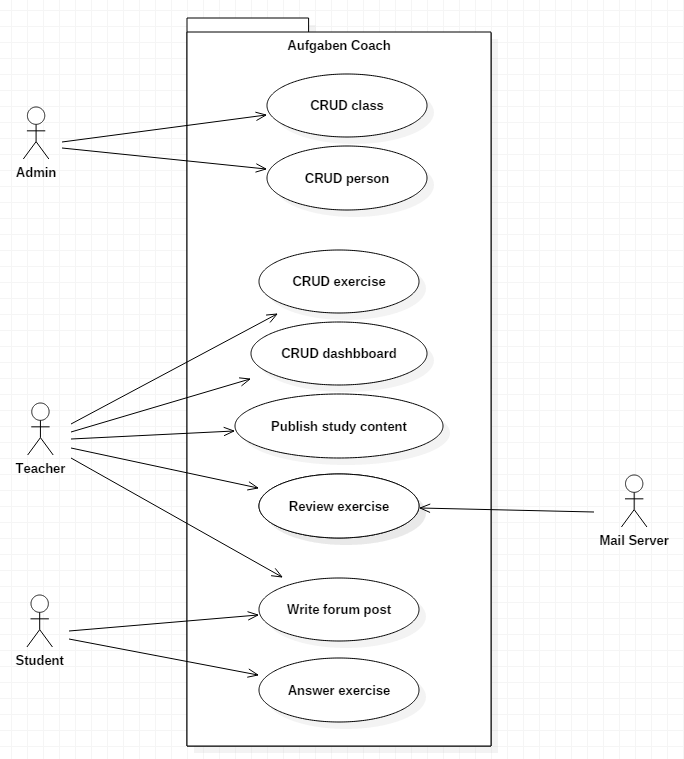
\includegraphics[width=\textwidth, height=\textheight, keepaspectratio]{images/UseCaseDiagramm.png}
	\caption{Use Case Diagramm}
	\label{uc_diagram}
\end{figure}

\end{minipage}


\subsubsection{Aktoren}
In der Tabelle \ref{aktoren} werden die Aktoren, welche mit der Anwendung interagieren, beschrieben. 
\begin{table}[H]
	\centering
	\begin{tabu} to 0.9\textwidth {l X}
	\toprule
	Aktor & Beschreibung \\ 
	\midrule
	Administrator & Der Administrator ist für die Verwaltung der Klassen, Lehrer und Schüler zuständig. Er kann Klassen erstellen sowie Lehrpersonen und Schüler diesen Klassen zuweisen. \\
	\midrule
	Lehrer & Der Lehrer verwaltet die ihm zugewiesenen Klassen. Er kann Fächer für seine Klassen freischalten sowie Aufgaben erstellen und diese der Klasse zuweisen. Zusätzlich kann er Statistiken einsehen, die ihn über den aktuellen Wissensstand seiner Klasse informieren. \\
	\midrule
	Schüler & Die Schüler haben Zugriff auf freigeschaltete Lerninhalte und können diese anschauen. Falls Fragen auftreten, können diese im aufgaben-spezifischen Forum gestellt werden. Zusätzlich können Aufgaben gelöst werden. \\
	\midrule
	Mail Server & Der Mail Server dient dem Versenden von Nachrichten, falls zum Beispiel eine Lehrperson ein Feedback an einen Lernenden schicken möchte. \\
	\bottomrule
	\end{tabu}
	\captionof{table}{Aktoren}
	\label{aktoren}
\end{table}


\subsubsection{Beschreibung der Use Cases}
\subsubsection*{CRUD person}

\begin{itemize}
	\item Hauptszenario:
	\begin{itemize}
		\item Der Administrator kann einen neuen Benutzer erstellen. Neue Benutzer können entweder die Rolle ''Schüler'' oder ''Lehrer'' haben.
	\end{itemize}
	\item Alternatives Szenario:
	\begin{itemize}
		\item Der Administrator entfernt eine Person aus dem System.
		\item Der Administrator ändert Angaben zu einer bereists existierenden Person. 
	\end{itemize}
\end{itemize}


\subsubsection*{CRUD school class}

\begin{itemize}
	\item Hauptszenario:
	\begin{itemize}
		\item Der Administrator erstellt eine neue Klasse, welcher Lehrpersonen und Schüler zugewiesen werden können.
	\end{itemize}
	\item Alternatives Szenario:
	\begin{itemize}
		\item Nach Ablauf eines Schuljahres kann der Administrator Klassen aus dem System entfernen.
		\item Der Administrator kann einzelne Schüler aus einer Klasse entfernen und diese einer anderen Klasse zuweisen.
	\end{itemize}
\end{itemize}


\subsubsection*{CRUD exercise}
\begin{itemize}
	\item Hauptszenario:
	\begin{itemize}
		\item Der Lehrer kann neue Aufgaben erstellen und diese einem Thema zuweisen. Pro Aufgabe gibt es mehrere Fragen, welche wiederum mehrere Hifestellungen enthalten können. Für jede Frage kann auch eine maximale Punktzahl angegeben werden. 
	\end{itemize}
	\item Alternatives Szenario:
	\begin{itemize}
		\item Der Lehrer passt einzelne Fragen oder Hilfestellungen an oder fügt neue Fragen einer Aufgabe hinzu.
	\end{itemize}
\end{itemize}



\subsubsection*{Assign exercise to weekly schedule}
\begin{itemize}
	\item Hauptszenario:
	\begin{itemize}
		\item Der Lehrer passt den Wochenplan einer Klasse an und fügt neue Aufgaben hinzu.
	\end{itemize}
	\item Alternatives Szenario:
	\begin{itemize}
		\item Der Lehrer verschiebt den Abgabetermin einer Aufgabe auf einen anderen Tag.
	\end{itemize}
\end{itemize}



\subsubsection*{Publish content}
\begin{itemize}
	\item Hauptszenario:
	\begin{itemize}
		\item Der Lehrer kann für einzelne Klassen die Fächer freischalten.
	\end{itemize}
	\item Alternatives Szenario:
	\begin{itemize}
		\item Freigeschaltene Fächer können wieder entfernt werden.
	\end{itemize}
\end{itemize}



\subsubsection*{View statistics}
\begin{itemize}
	\item Hauptszenario:
	\begin{itemize}
		\item Der Lehrer kann die Statistiken einzelner Klassen oder Schüler ansehen. Diese Ansicht zeigt dem Lehrer, auf welchem Wissensstand eine Klasse oder einzelne Schüler sind.
	\end{itemize}
\end{itemize}


\subsubsection*{Create forum post}
\begin{itemize}
	\item Hauptszenario:
	\begin{itemize}
		\item Treten beim Lösen von Aufgaben Unklarheiten auf, kann ein Schüler eine entsprechende Frage direkt im aufgabenspezifischen Forum stellen.
	\end{itemize}
	\item Alternatives Szenario:
	\begin{itemize}
		\item Ein Schüler sieht eine Frage im Forum, zu welcher er die Lösung weiss. Er kann auf den Beitrag seines Schulkameraden antworten und ihm so helfen.
	\end{itemize}
\end{itemize}


\subsubsection*{Send mail}
\begin{itemize}
	\item Hauptszenario:
	\begin{itemize}
		\item Der Lehrer hat die Möglichkeit, gelöste Aufgaben an die Schüler zurückzuweisen. Ist dies der Fall, wird eine E-Mail mit dem Feedback des Lehrers an den Schüler gesendet.
	\end{itemize}
\end{itemize}


\subsubsection*{Solve exercise}
\begin{itemize}
	\item Hauptszenario:
	\begin{itemize}
		\item Der Schüler kann die Aufgaben von freigegebenen Fächern lösen. Sind alle Fragen beantwortet, kann die Übung abgegeben und vom Lehrer korrigiert werden.
	\end{itemize}
	\item Alternatives Szenario:
	\begin{itemize}
		\item Falls der Lehrer die Übung eines Schülers zurückweist, kann dieser die Fragen nochmals überarbeiten.
	\end{itemize}
\end{itemize}


\subsection{Nicht Funktionale Anforderungen}
Bei der Erstellung der einzelnen \gls{nfr} wird auf FURPS zurückgegriffen. FURPS ist ein Akronym für Functionality, Usability, Reliability, Performance und Supportability. Dieses Modell wurde im Jahre 1992 von HP entwickelt und dient zur Priorisierung der Software Requirements.\footcite{furps_description}

\begin{table}[h]
	\centering
	\begin{tabu} to 0.9\textwidth {l l X}
	\toprule
	FURPS & Titel & Beschreibung \\ 
	\midrule
	Functionality & User Interface & Das User Interface der Applikation ist über den Webbrowser erreichbar. \\ 
	& Security & Die einzelnen Benutzer können nur auf die für sie freigegebenen Inhalte zugreifen. \\
	& HTTPS & Die Kommunikation zum Webserver soll über HTTPS laufen. \\
	\midrule
	Usability & Responsiveness & Für Schüler soll die Applikation sowohl auf Desktop PCs wie auch auf Tablets oder Mobile Phones verfügbar sein. \\
	\midrule
	Reliability & Availability & Die Applikation soll zu 95\% des Tages verfügbar sein. \\
	 & Fault Tolerance & Die Applikation soll bei unerlaubten Anfragen weiterhin verfügbar sein. \\
	\midrule
	Performance & Response Time & Wechselt der Benutzer zwischen einzelnen Seiten, soll die neue Seite in maximal einer Sekunde geladen werden.\\
	\midrule
	Supportability & Maintainability & Die Applikation soll so gebaut werden, dass sie auch in Zukunft gewartet und ausgebaut werden kann. \\
	 & Scalability & Die Applikation soll von 300 Benutzern zeitgleich verwendet werden können. \\
	\bottomrule
	\end{tabu}
	\captionof{table}{Non Functional Requirements}
\end{table}

%\subsubsection{Functionality}
%\subsubsection*{}
%
%\subsubsection{Qualität}
%Um die Qualität des Codes möglichst hoch zu halten und sicherzustellen, dass alle Teammitglieder immer auf dem aktuellsten Stand sind, werden auf Git Pull-Requests verwendet. Dadurch kann sichergestellt werden, dass ein anderes Teammitglied den geschriebenen Code ebenfalls angesehen und durchdacht hat.
%
%\subsubsection*{Maintainability}
%Die Software könnte unter Umständen in einem Start-Up verwendet werden. Da in Zukunft noch beinahe beliebig viele neue Anforderungen hinzustossen können, soll die Applikation so gebaut werden, dass sie einfach modifiziert werden kann. 
%
%\subsubsection*{Reliability}
%Die Applikation soll robust und reibungslos laufen, auch wenn mehere Schüler zeitgleich mit der Plattform verbunden sind.
%
%\subsubsection*{Scalability}
%Das System soll problemlos von bis zu 300 Benutzern gleichzeitig verwendet werden können. 
%
%\subsubsection*{Usability}
%Bei der Applikation soll es sich um eine Mobile First Applikation handeln. Die Plattform soll sowohl auf Desktop PCs, Tablets und Smartphones bedienbar sein. Der Lehrer- und Administator-spezifische Teil der Applikation ist davon erstmals ausgenommen, da davon ausgegangen wird, dass diese beiden Aktoren hauptsächlich auf Desktop PCs arbeiten. 
%Die Applikation soll ein intuitives User Interface besitzen, damit sich die Benutzer auf Anhieb zurechtfinden. 
%
%\subsubsection*{Security}
%Der Zugriff auf das System ist passwortgeschützt. Benutzer können sich nicht selbstständig registrieren. Nur Administratoren können neue Benutzer erfassen.
%Jede Person sieht nur die Informationen, die für sie selbst von Bedeutung sind. Ein Schüler hat zum Beispiel keinen Zugriff auf die Statistiken anderer Schüler.


\newpage